\chapter{使い方}

\section{行間表記の入力}

\subsection{はじめに}

 TuneEditorはウィンドウ上部に数多くのボタン類を配置しているため、編集領域が狭くなってしまっています。このため使用に先立って、ブラウザーの表示縮小コマンドを用いて表示サイズを縮小しておくのがおすすめです。

\subsection{テキストの入力}

 テキストの入力は通常のエディターと同様であり、キーボードから入力した文字がそのままテキスト領域に表示されていきます。そして、その入力に合わせて行間表記のドットが自動的に追加されていきます。なお、ドットの追加規則は以下の通りです。

\begin{itembox}[l]
{\textsf{ドットの追加規則}}\label{dottingRules}

\begin{itemize}
\item 入力した文字が\textsf{音節核候補文字}(``aeiouy''というアルファベット6文字(大文字および小文字)と、``{\tnr{ɨʉɯɪᵻᵿʊøɘɵɤəɛœɜɞʌɔæɐɶɑɒɚ}}''という国際音声記号(IPA)24文字)である場合、直前および直後にある文字の\textsf{双方}が音節核候補文字\textsf{以外}の文字であれば、該当位置にドットを挿入します。

\bigskip
\item 入力した文字が音節核候補文字\textsf{以外}である場合、直前および直後にある文字の\textsf{双方}が音節核候補文字であれば、該当位置の次の文字位置にドットを挿入します。
\end{itemize}
\bigskip
※ なお、行頭の直前、そして行末の直後には架空の\textsf{非}音節核候補文字があると想定して動作します。
\end{itembox}


\subsection{他のアプリでコピーした文字(群)のペースト}

 他のアプリでコピーした文字(群)をペーストするには、以下の操作を実行します。\label{copyPaste}

\begin{quote}
\begin{enumerate}
\item TuneEditorの画面右上にある水色の領域をクリックして、ピンク色に変える。
\item その状態で、\texttt{command+V}(macOSの場合)、または\texttt{Ctrl+V}(WindowsやLinuxの場合)を押下する。
\end{enumerate}
\end{quote}

なお、いったんピンク色に変えた状態で、ペースト処理を中止したい場合には、画面上の他の領域をクリックすれば、領域は水色に戻ります。

\begin{itembox}[l]
{\textsf{コピー&ペースト操作に関する舞台裏の話}}
 TuneEditorのようなブラウザー上で動作するウェブアプリには、コピー&ペースト機能に厳しい制限が課されています。というのも、ウェブアプリは、ウェブサイトにアクセスするだけで自動的に実行されるようになっているため、コピー&ペーストに何らかの制限を課しておかなければ、ユーザーがデリケートな情報(パスワードや個人情報など)をクリップボードにコピーしている状態で、悪意のあるURLにアクセスした場合、あっという間にその情報が犯罪者たちのもとに送信されてしまうためです。

\bigskip
 この制限ゆえに、ウェブアプリ内で実行するコピー&ペースト処理は通常のコピー&ペースト操作とは異なり、ユーザーの許可を必要とするようになっています。しかも標準化策定の遅れもあって、2022年6月時点ではすべてのブラウザーで標準APIが実装されるに至っていません。

\bigskip
 このため、TuneEditorではコピー&ペースト用の標準APIを用いるのではなく、ブラウザーがあらかじめ用意している、画面作成用の部品を利用してウェブアプリ内にクリップボードの内容を送り込むという方式を採用しています。

\bigskip
 早い話、ウィンドウ右上の水色/ピンク色の領域は、HTMLレベルで用意されている単なるテキスト領域(\texttt{TEXTAREA})です(テキスト領域へのペーストは、従来のコピー&ペーストと同じ操作が可能になっているのです)。ただ、このテキスト領域はフォーカスが当たっていない時には背景色、文字色ともに水色に、フォーカスが当たっている時には背景色、文字色ともにピンク色になるよう設定しています(つまり単なる「インジケーター」兼データの入れ物として使っています)。そして、この領域に入力があった場合、TuneEditorは文字(群)が入力されたと判断し、その内容を取り込むようになっているのです。

\end{itembox}


\subsection{国際音声記号(IPA)や全角文字などの特殊な文字の入力}

 TuneEditorはキーボードの押下を直接読み取って動作するため、キーボード上に刻印されている文字以外を入力することはできません。つまり、国際音声記号(IPA)やかな漢字変換の結果(つまり漢字などの全角文字)を入力することはできません。

そういった文字を入力するには、他のアプリケーション上で作成した文字(群)をコピー&ペーストによって入力することになります。操作の詳細は\pageref{copyPaste}ページを参照してください。


\subsection{ドットの大きさと高さの指定}

 ドットの大きさと高さを指定するには、ウィンドウ上部の\texttt{Stress}という見出しの下にある3x9列のボタン群を使用します。操作方法は以下の通りです。

\begin{quote}
\begin{enumerate}
\item 指定したいドットをクリックすると、そのドットの表示色が赤くなり、フォーカスが当たる\footnote{もう一度クリックするとフォーカスは外れます。}とともに、テキストカーソルも対応付けられている音節核候補文字の先頭に移動します。
\item 必要なドットサイズ(大/中/小のいずれか)と高さに該当するボタンを押します。
\end{enumerate}
\end{quote}

なお、ボタンを押下すると、次のドットにフォーカスが移動します。この移動を抑止したい場合には、\texttt{Shift}キーを押しながらボタンを押してください。

また、直前のドットにフォーカスを移動させたい場合には\texttt{command+Z}(macOS使用時)、または\texttt{Ctrl+Z}(WindowsまたはLinux使用時)を押下するか、ウィンドウ画面上部の[◀]をクリックしてください。

さらに、直後のドットにフォーカスを移動させたい場合には\texttt{command+shift+Z}(macOS使用時)、または\texttt{Ctrl+Shift+Z}(WindowsまたはLinux使用時)を押下するか、ウィンドウ画面上部の[▶]をクリックしてください。

\begin{figure}[htbp]
\begin{center}
	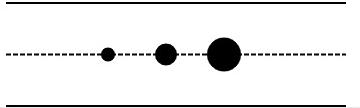
\includegraphics[width=4cm]{DotsSize.png}
	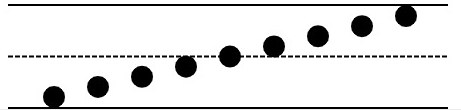
\includegraphics[width=5cm]{DotsHeight.png}
 \end{center}
 \label{sampleImage}
\end{figure}



\subsection{音調核でのイントネーション変化を指定する}

 ドットには、音調核の単音節内でのピッチ移動を表現するために5種類\footnote{TSMでは7種類の記号が用意されていますが、Low-FallとHigh-Fall、そしてLow-RiseとHigh-Riseはドット自体のピッチの高さで区別できるため、5種類となっています。}の「尻尾」を付加することができます。これにはToneという見出しの下にある6つのボタンを使用します。

\begin{quote}
\begin{description}
\item[Low/High−Fall]:下降ピッチ
\item[Rise−Fall]:上昇後下降ピッチ
\item[Low/High−Rise]:上昇ピッチ
\item[Fall-Rise]:下降後上昇ピッチ
\item[Mid-Level]:平坦ピッチ
\item[-cancel pattern-]:ピッチ無し(リセット)
\end{description}
\end{quote}

\begin{figure}[htbp]
\begin{center}
	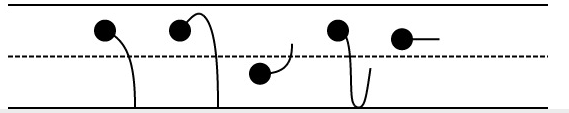
\includegraphics[width=8cm]{DotsNucleus.png}
 \end{center}
 \label{sampleImage}
\end{figure}


なお、ドットの大きさと高さを変更するボタンを押した場合、ドットのフォーカスは自動的に次のドットに移り、そのドットが赤色で表示されますが、この操作の直後にピッチ移動ボタンを押した時に限り、ピッチ移動の適用対象は今高さと大きさを指定したドットになります。それ以外の場合は、まず適用対象のドットをマウスでクリックした上で、ピッチ移動ボタンを押してください。

\subsection{ドットを移動する}

 ドットの移動はマウスのドラッグで可能です。

\subsection{ドットを非表示にする、または表示状態に戻す}

 TuneEditorでは入力した文字のパターンに従って、ドットを追加するようになっています。このため、例えば``cake''といった1音節の単語を入力した場合であっても、2文字目の``a''に対応した適切なドットと、4文字目の``e''に対応した不要なドットが表示されてしまいます。こういった不要なドットを非表示にするには、以下の手順を実行します。

\begin{quote}
\begin{enumerate}
\item 非表示にしたいドットをクリックし、赤色で表示させます。
\item [Make item invisible]ボタンを押します。
\end{enumerate}
\end{quote}


また、いったん非表示にしたドットは、以下の手順で表示状態に戻すことができます。

\begin{quote}
\begin{enumerate}
\item [Make item visible again]ボタンを押すと、非表示にしたドット(群)が青色で表示されます。
\item 表示状態に戻したいドットをクリックします。
\end{enumerate}
\end{quote}

\subsection{新たにドットを追加する}

 TuneEditorでは入力した文字の種類と組み合わせに従って、ドットを追加するようになっています。このため、例えば``10''と入力した場合にはどこにも音節核候補文字がないため、ドットが表示されません。こういったケースに対応するための、以下のような姑息な(!)手段が用意されています。

\begin{quote}
\begin{enumerate}
\item ドットを追加したい場所の近傍にある、音節核候補文字\textsf{ではない}文字が2つ連続している場所を見つけ出します。
\item それら文字の\textsf{間}でマウスをクリックし、テキストカーソルを移動した後、[esc]キーを押してコマンドメニューを表示させ、「\texttt{aa}」(Add A Toneコマンド)と入力します。
\end{enumerate}
\end{quote}


\begin{itembox}[l]
{\textsf{音節核候補文字のない場所でのドット表示}}
 TuneEditorでは音節核候補文字のない場所でドットを表示させるため、「テキスト上は表示されない、すなわち\textsf{横幅がゼロ}の文字を用意して、この文字を音節核候補文字として扱うようにしています。そして、[esc]-「\texttt{aa}」コマンドでその文字を入力するようにしています。

\bigskip
 つまり、音節核候補文字ではない文字の並びの間に「表示されない音節核候補文字」を挿入することで、ドットが追加されるように仕向けているのです。

\bigskip
 このやり方の弊害として、テキストカーソルを矢印キーで1文字ずつ移動させると、表示されない文字のある部分で、カーソルが足踏みするように見えるという点があります(許してください)。
\end{itembox}


\subsection{中央線を表示する、または非表示にする}

 行間表記の中間にデフォルトで描画される破線は、ウィンドウ上部の[Centreline]チェックボックスを用いて表示/非表示を切り替えることができます。

この中央線を描画するというアイデアは、長瀬慶來先生より久保岳夫先生経由で頂いたコメントに基づいております。この場を借りて感謝いたします。

\subsection{区切り線を追加する}

 行間表記領域には8種類の区切り線を追加することができます。これらはマウスのドラッグで移動でき、ドットと同様の操作で非表示にしたり、再表示させることができます。

行間表記の区切り線は8種類をサポートしており、以下のようにして入力します。

\begin{quote}
\begin{enumerate}
\item ウィンドウ上部の[Separator (Solid line)](実線表示)または[Separator (Dashed line)](破線表示)をマウスでクリックする。
\item 区切り線を入力したいところでマウスをクリックする。
\end{enumerate}
\end{quote}

なお、マウスをクリックする際に「\texttt{shift}」キー(二重線)や、「\texttt{option}」キー(三重線)、「\texttt{shift}+\texttt{option}」キー(変則二重線)を押すことで区切り線の形状を変えることができます。

\medskip
\begin{center}
	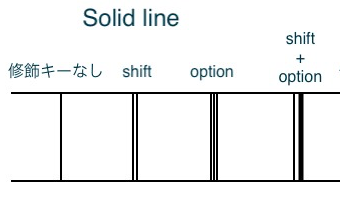
\includegraphics[width=6cm]{SolidLine.png}\label{SolidLineSample}
	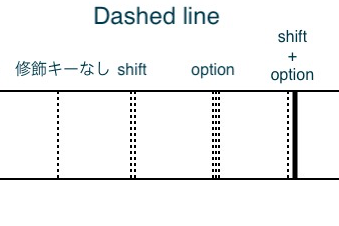
\includegraphics[width=6.2cm]{DashdLine.png}\label{DashedLineSample}
 \end{center}
\medskip


\textsf{注意点:}なおTuneEditor Ver. 4.01では、区切り線の位置管理を文字種別とは独立したかたちで行うようになったため、テキスト内容を変更しても、その変更に追随して区切り線の描画場所がシフトしていくようにはなっていません(気が向けば対応します)。


\newpage
\section{TSMの入力}

 TSMはテキスト領域に付加していく記号です。行間表記は不要でTSM表記のみ必要だという場合、ウィンドウ上部にある[Use Graphics]チェックボックスのチェックを外してください。

\subsection{各種記号の入力}

 TuneEditorでは以下のTSM記号をサポートしており、すべて「\texttt{esc}」キーを押下した際に表示されるコマンドメニューから行えるようになっています。

\begin{center}
	
\includegraphics[width=12cm]{TSMsymbols.jpeg}
 \end{center}

また、公式に定義されていないLow-Prehead記号(``\_'')や、複数の区切り線のバリエーションも使用できます。

\begin{center}
	\includegraphics[width=12cm]{additionalSymbols.jpeg}
 \end{center}


なお、「\texttt{esc}」キーで表示されるメニューは、もう一度「\texttt{esc}」キーを押すか、2文字を入力すると閉じ、その2文字がコマンドとして定義されている場合に、該当コマンドを実行します。

以下は、公式のTSM記号を入力する際に用いるコマンドの一覧です。

\renewcommand{\arraystretch}{1.2}
\begin{table}[h]
	\centering
	\begin{tabular}{ccl}
	\hline
	記号 & コマンド & 意味\\
	\hline
	\hline
	 ̄ & HP & 高前頭部\\
	\hline
	ˈ & H1 & 高い音の強勢\\
	\hline
	゜ & H2 & 高い音の準強勢\\
	\hline
	\tiny{$^↘$} & H3 & 下降調\\
	\hline
	ˌ & L1 & 低い音の強勢\\
	\hline
	。 & L2 & 低い音の準強勢\\
	\hline
	\tiny{$_↗$} & L3 & 上昇調\\
	\hline
	\hline
	$^\$ & HF & 高下降調(音調核)\\
	\hline
	$^/$ & HR & 高上昇調(音調核)\\
	\hline
	$_\$ & LF & 低下降調(音調核)\\
	\hline
	$_/$ & LR & 低上昇調(音調核)\\
	\hline
	$^∧$  & RF & 上昇下降調(音調核)\\
	\hline
	$^∨$ & FR & 下降上昇調(音調核)\\
	\hline
	$^>$ & ML & 平坦調(音調核)\\
	\hline
	\hline
	| & IP & イントネーション句の区切り\\
	\hline
	‖ & FS & イントネーション句の区切り(文末等)\\
	\hline
	\end{tabular}
\end{table}

非公式な記号を入力するコマンドは、メニューに表示されていませんが、次のようになっています。

\begin{quote}
\begin{description}
\item[lp] 低前頭部の記号です(これは高前頭部との違いを際立たせたい特殊な場合にしようできます)
\item[i0, i1, i2, i3] 区切り線の上に赤で「0〜3」の数字を追記した記号です
\item[s1, s2, s3, s4] 実線の区切り線で、行間表記の区切り線の4パターンに対応した記号です(\pageref{SolidLineSample}ページを参照)。
\item[d1, d2, d3, d4] 破線の区切り線で、行間表記の区切り線の4パターンに対応した記号です(\pageref{DashedLineSample}ページを参照)。
\end{description}
\end{quote}

\begin{table}[h]
	\centering
	\begin{tabular}{cl}
	\hline
	コマンド & 意味\\
	\hline
	\hline
	LP & 低前頭部記号(高前頭部との違いを際立たせたい場合に使用)\\
	\hline
	i0 & 実線の区切り線の上に赤で「0」を表示したもの\\
	i1 & 実線の区切り線の上に赤で「1」を表示したもの\\
	i2 & 実線の区切り線の上に赤で「2」を表示したもの\\
	i3 & 実線の区切り線の上に赤で「3」を表示したもの\\
	\hline
	s1 & 実線の区切り線(「\texttt{IP}」と同じ)\\
	s2 & 実線の区切り線(「\texttt{FS}」と同じ)\\
	s3 & 実線の区切り線(3重線)\\
	s4 & 実線の区切り線(変則2重線)\\
	\hline
	d1 & 破線の区切り線(1本線)\\
	d2 & 破線の区切り線(2重線)\\
	d3 & 破線の区切り線(3重線)\\
	d4 & 破線の区切り線(変則2重線)\\
	\hline
	\end{tabular}
\end{table}


\subsection{下線の引き方}

 以下の手順で下線を引くことができます。

\begin{quote}
\begin{enumerate}
\item 以下のいずれかの方法で、下線を引きたい部分を選択する。
	\begin{itemize}
	\item 選択範囲の一方の端にテキストカーソルを置き、「\texttt{Shift}」キーを押しながら、矢印キーを押して選択範囲を広げていく。
	\item テキスト領域をマウスでドラッグする。
	\item 選択範囲の一方の端にテキストカーソルを置き、「\texttt{Shift}」キーを押しながら、もう一方の端をマウスでクリックする。
	\end{itemize}
\item 「\texttt{esc}」キーを押した後、「\texttt{su}」(Set Underline)と入力する。
\end{enumerate}
\end{quote}

\subsection{下線の消し方}

 いったん引いた下線は、下線を引いた際と同じ方法で下線を消去したい領域を選択し、「\texttt{esc}」キーを押した後、「\texttt{cu}」(Clear Underline)と入力することで消去できます。

\subsection{その他の注意点}

 テキスト行のコピー&ペーストは、ブラウザー上のTuneEditorインスタンスが実行されているタブ内でしか実行できません。またその際には、TSM記号をコピーすることはできません(記号部分は空白として処理されます)。
